\documentclass{../cssheet}


%--------------------------------------------------------------------------------------------------------------
% Basic meta data
%--------------------------------------------------------------------------------------------------------------

\title{Noch mehr folgenreiche Aufgaben}
\author{Prof. Dr. Christian Spannagel}
\date{\today}
\hypersetup{%
    pdfauthor={\theauthor},%
    pdftitle={\thetitle},%
    pdfsubject={Aufgabenblatt Inside Math!},%
    pdfkeywords={insidemath}
}

%--------------------------------------------------------------------------------------------------------------
% document
%--------------------------------------------------------------------------------------------------------------

\begin{document}
\printtitle


\textbf{Aufgabe 1 (Musteranalyse):}  Analysiert die Figurenfolgen.
\begin{enumerate}[a)]
\item Wie geht es jeweils weiter? 
\item Aus wie vielen Streichhölzern / Punkten besteht die $100.$ Figur? 
\item Welche Figur besteht aus $100$ Streichhölzern / Punkten? Warum?
\item Gebt für die Folgen jeweils die rekursive und die geschlossene (explizite) Form an.
\end{enumerate}

\begin{center}
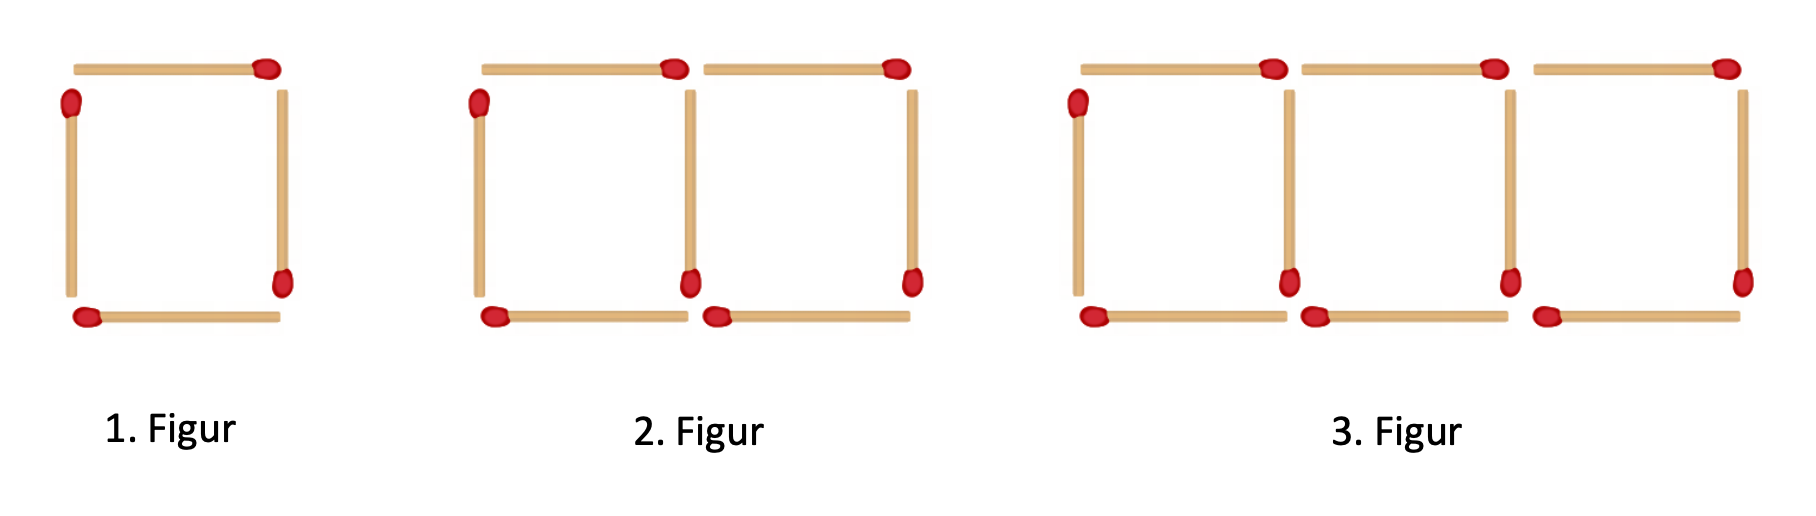
\includegraphics[width=12cm]{streichhoelzer.png}
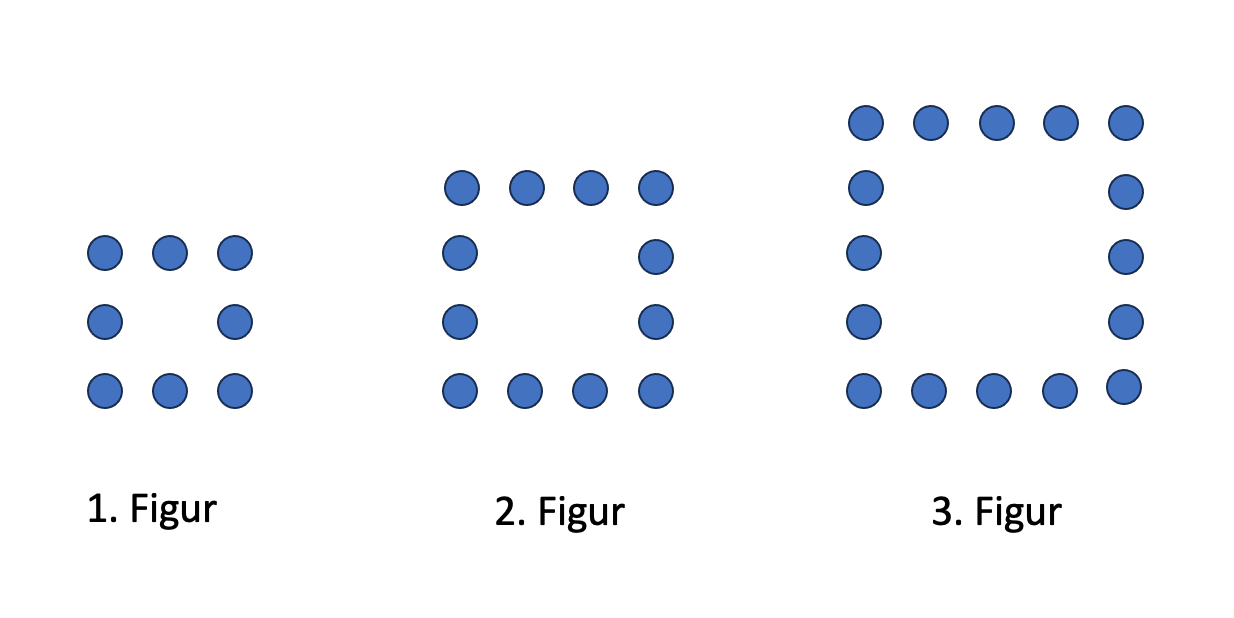
\includegraphics[width=10cm]{punktemuster.png}
\end{center}


\textbf{Aufgabe 2 (Wir addieren Nachbarn):}  Was passiert, wenn ihr zwei aufeinander folgende
Dreieckszahlen miteinander addiert? Begründet das auf verschiedene Weisen (mit einem
Bild, mit einer Formel, \ldots).


\textbf{Aufgabe 3 (Versteckspiel):}  Nehmt euch verschiedene Dreieckszahlen her, multipliziert sie mit $8$ und addiere jeweils $1$. Auch hier wieder: Fällt euch etwas auf? Könnt ihr das begründen?) 


\vspace*{10mm}
\printlicense

\printsocials



\end{document}
